% !TEX TS-program = LuaLaTeX
\documentclass[11pt,compress,xcolor=x11names,UTF8]{beamer}
\usetheme{Boadilla}
\usecolortheme{seahorse}
\useinnertheme[shadow]{rounded}  
\useoutertheme[subsection=false]{smoothbars}
\usecolortheme{spruce}
\usecolortheme[named=SpringGreen4]{structure}
\usefonttheme{structurebold}
\useinnertheme{circles}
\usecolortheme{rose}
\usepackage{pifont}
\usepackage{academicons}
\usepackage{fontawesome}
\usepackage{iitem}
%\usepackage{graphicx}
%\usepackage{tabular}
\setbeamertemplate{itemize item}{\ding{108}}
\setbeamertemplate{itemize subitem}{\ding{109}}
\setbeamertemplate{navigation symbols}{}
\setbeamercovered{transparent}  
\renewcommand\appendixname{附录}
\renewcommand\abstractname{摘要}
\graphicspath{{figure/}} % 图片路径
\usepackage{calligra} % Thank you
\usepackage{ctex} % 加入中文
%\setCJKsansfont{Noto Sans CJK SC}
\setsansfont{Lato} % Lato Roboto Fira Sans
\usepackage{makecell}
\newcommand{\tabincell}[2]{\begin{tabular}{@{}#1@{}}#2\end{tabular}}
\usepackage{url}					
\usepackage{natbib} % 参考文献
%\title[Spatial Generalized Linear Mixed Models]{Spatial Generalized Linear Mixed Models with Application to Prevalence Mapping}
\title{PMT layout and orientation in CD}
%\subtitle{奖助金申请答辩}
\author[Rong. Zhao]{Email:zhaor25@mail2.sysu.edu.cn \and  } % \\ 专业:统计学 \\ 方向:数据分析与统计计算
\institute[Sun Yat-Sen University]{School of Physics\and } % 理学院\\
\date[\today]{\includegraphics[width=.5\textwidth]{logo}}

\begin{document}

\maketitle

%\begin{frame}{Outline}
%\tableofcontents
%\end{frame}

\section{PMT layout}

%\subsection{研究意义}

\begin{frame}{PMTs}
%\textsf{例} \textbf{例}  \textit{例} 
% \texttt{例}  % 调出仿宋字体了
We have two types of PMT:\\ HAMAMATSU (about 5k)\& NNVT(about 15k), in general:
\begin{table}[]  
\caption{PMT typical performance}  
%\resizebox{.8\textwidth}{!}{%
\begin{tabular*}{.98\textwidth}{l|cccc}
%\toprule  
\hline  
\hline  
Performance & PDE &DCR & TTS& uniformity \\  
\hline  
HAMAMATSU &  lower\% & 20 kHz& 3ns& worse \\  
NNVT  & higher\% & 40kHz & 7ns& better \\  
\hline  
\end{tabular*}  
%}
\end{table} 
%\begin{figure}
%\centering
%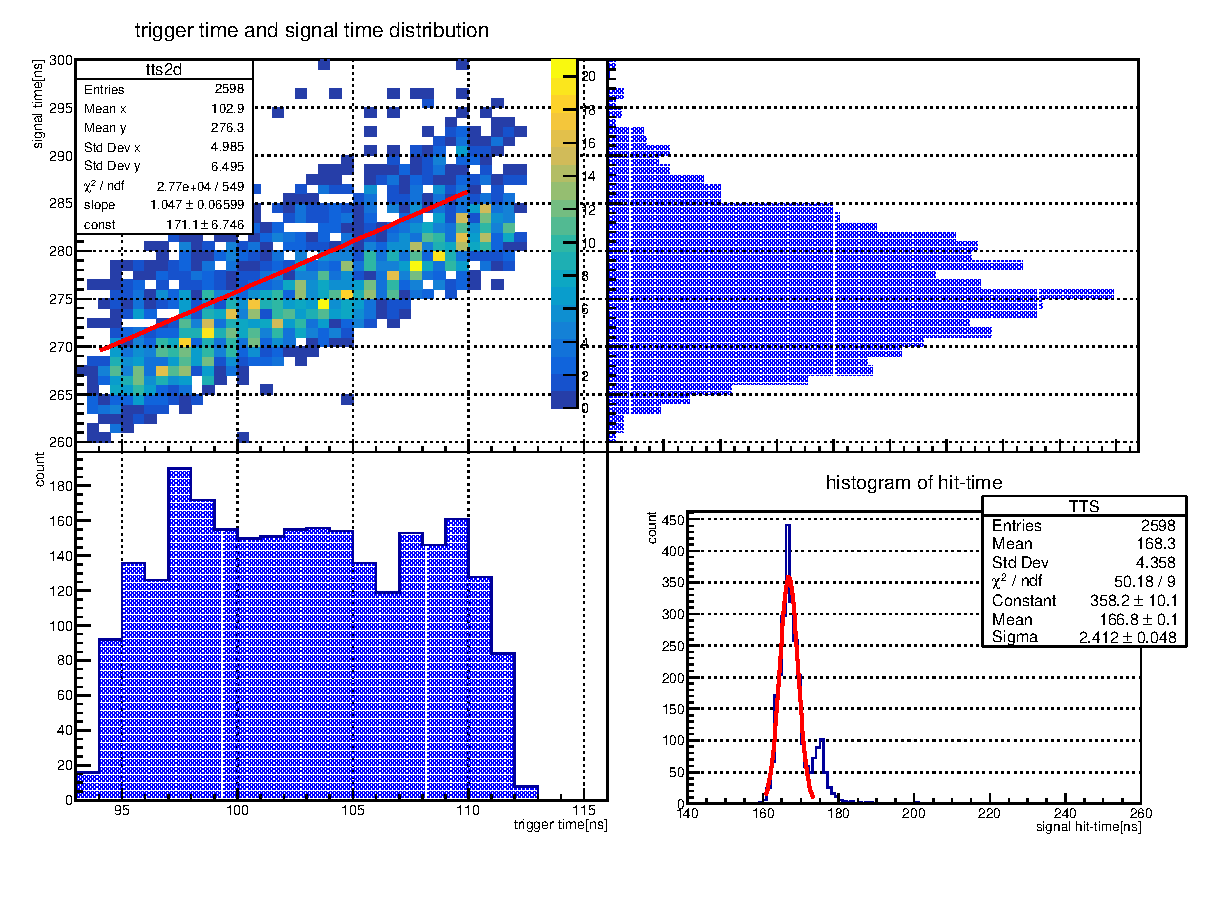
\includegraphics[width=0.78\textwidth]{typical_hittime} % 单图
%\end{figure}

\end{frame}
%%%%%%%%%%%%%%%%%%%%%%%%%%%%%%%%%%%%%%%%%%%
\begin{frame}{patterns}
\begin{figure}
\centering
\includegraphics[width=0.78\textwidth]{random} % 单图
\end{figure}

\end{frame}
%%%%%%%%%%%%%%%%%%%%%%%%%%%%%%%%%%%%%%%%%%%
\begin{frame}{patterns}
\begin{figure}
\centering
\includegraphics[width=0.58\textwidth]{pat1} % 单图
\end{figure}

\end{frame}
%%%%%%%%%%%%%%%%%%%%%%%%%%%%%%%%%%%%%%%%%%%
\begin{frame}{patterns}
\begin{figure}
\centering
\includegraphics[width=0.58\textwidth]{pat2} % 单图
\end{figure}

\end{frame}
%%%%%%%%%%%%%%%%%%%%%%%%%%%%%%%%%%%%%%%%%%%
\begin{frame}{patterns}
\begin{figure}
\centering
\includegraphics[width=0.58\textwidth]{pat3} % 单图
\end{figure}

\end{frame}
%%%%%%%%%%%%%%%%%%%%%%%%%%%%%%%%%%%%%%%%%%%
\begin{frame}{patterns}
\begin{figure}
\centering
\includegraphics[width=0.58\textwidth]{pat4} % 单图
\end{figure}

\end{frame}
%%%%%%%%%%%%%%%%%%%%%%%%%%%%%%%%%%%%%%%%%%%
\begin{frame}{patterns}
\begin{figure}
\centering
\includegraphics[width=0.58\textwidth]{pat5} % 单图
\end{figure}

\end{frame}
%%%%%%%%%%%%%%%%%%%%%%%%%%%%%%%%%%%%%%%%%%%
\begin{frame}{patterns}
\begin{figure}
\centering
\includegraphics[width=0.58\textwidth]{pat6} % 单图
\end{figure}

\end{frame}
%%%%%%%%%%%%%%%%%%%%%%%%%%%%%%%%%%%%%%%%%%%
\begin{frame}{patterns}
\begin{figure}
\centering
\includegraphics[width=0.58\textwidth]{pat7} % 单图
\end{figure}

\end{frame}
%%%%%%%%%%%%%%%%%%%%%%%%%%%%%%%%%%%%%%%%%%%
\begin{frame}{patterns}
\begin{figure}
\centering
\includegraphics[width=0.58\textwidth]{pat8} % 单图
\end{figure}

\end{frame}

%%%%%%%%%%%%%%%%%%%%%%%%%%%%%%%%%%%%%%%%%%%%%%%%%%%%%%%%%%%%%%%%%%%%
\begin{frame}{ JUNO offline}
compare detector performance with the different PMT paterns, especially the time and energy resolution and reconstruction results.

\hrule{\textwidth}

how to:add method to the PMT class then each PMT can get its performance according to the layout pattern and its own ID. 
\end{frame}
%%%%%%%%%%%%%%%%%%%%%%%%%%%%%%%%%%%%%%%%%%%%%%%%%%%%%%%%%%%%%%%
\section{PMT orientation}
%%%%%%%%%%%%%%%%%%%%%%%%%%%%%%%%%%%%%%%%%%%%%%%%%%%%%%%%%%%%%%%%%%%%
\begin{frame}{HAMAMATSU PMTs}
the PDE uniformity of HAMAMATSU PMTs are not so good
\hrule{\textwidth}
we can artificially correct the PDE if these PMTs have fixed orientation and we can extract the light incident angle using reconstraction information.
\end{frame}
%%%%%%%%%%%%%%%%%%%%%%%%%%%%%%%%%%%%%%%%%%%%%%%%%%%%%%%%%%%%%%%


\begin{frame}
\centering {\zihao{0} \color{red} \calligra{Thank You}}

\end{frame}


%\begin{frame}[allowframebreaks]
%\frametitle{References}
%\scriptsize
%\bibliographystyle{authordate1}
%\bibliography{R-GLMM-pkgs}
%\end{frame}

\appendix

\section*{附录}

%\begin{frame}{Softwares and Tools}

%\includegraphics[width=.2\textwidth]{software/r}\qquad
%\includegraphics[width=.16\textwidth]{software/stan} \\ 
%\includegraphics[width=.45\textwidth]{software/bioconductor}
%\includegraphics[width=.45\textwidth]{software/PyMC3} 

%\end{frame}
%% OpenBUGS  WinBUGS  JAGS
% library(R2OpenBUGS) # 2017-2-20 version 3.2-3.2
% library(R2WinBUGS) # 2015-07-29 version 2.1-21
% library(rjags) # 2016-02-19 version 4-6
% library(BRugs) # OpenBUGS 2017-06-26  version 0.9-0
% library(glmmBUGS) # Generalised Linear Mixed Models with BUGS and JAGS 2016-09-22 version 2.4.0
% library(R2jags) # Using R to Run 'JAGS'  2015-08-23	 version 0.5-7

% network
	% diagram DiagrammeR DiagrammeRsvg
 % library(help=graph)

 % library(help=Rgraphviz)
 % library(help=igraph)


%\begin{frame}{Ack}
%\begin{itemize}
%\item[\faGithub] \href{https://github.com/Cloud2016}{Cloud2016} \faAt Github
%\item[\aiOverleaf] \href{https://www.overleaf.com/}{Xiangyun} \faAt Overleaf
%\item[\aiarXiv] \href{https://arxiv.org/}{arXiv}
%\end{itemize}
%\end{frame}

\end{document} 


